\chapter{Synchronization and coordination in distributed systems}
One of the main goal of DS is that for a set of process to synchronize and to coordinate their actions or to agree on one or more values.

Before introducing the algorithms we have to make an important distinction on synchronization:
\begin{itemize}
    \item \textbf{Internal:} agreement of a set of processes
    \item \textbf{External:} forced by an external agent
\end{itemize}

In distributed system there are several problem to analyse:
\begin{itemize}
    \item Clock Synchronization
    \item Mutual exclusion
    \item Election algorithm
    \item Atomic transaction
    \item Deadlock management
\end{itemize}

\section{Mutual Exclusion}
It can be considered as the \textbf{coordination activity} among a set of processes to share resources and keep consistency in the distributed system. \textbf{Distributed mutual exclusion} of a set of resources is characterised by three main features:
\begin{itemize}
    \item \textbf{Safety:} at most one process at time executes the critical section
    \item \textbf{Liveness:} A process that asks to enter in a critical section eventually enters it and at the end it leaves it
    \item \textbf{Ordering:} entering a critical section occurs some accord to the casual ordering
\end{itemize}

\section{Central Server Algorithm}
It has a simple implementation, \textbf{it simulates the primitives offered by the centralized server} through a coordinator process. Its behaviour is structured as follow:
\begin{enumerate}
    \item A process asks the coordinator to enter and it is possibly blocked
    \item The answer is an access \textbf{token}
    \item At receiving time of the answer, it enters the \textbf{critical section}
    \item At the \textbf{exit time} from the critical section it communicates to the coordinator 
\end{enumerate}

\begin{figure}[!h]
    \centering
    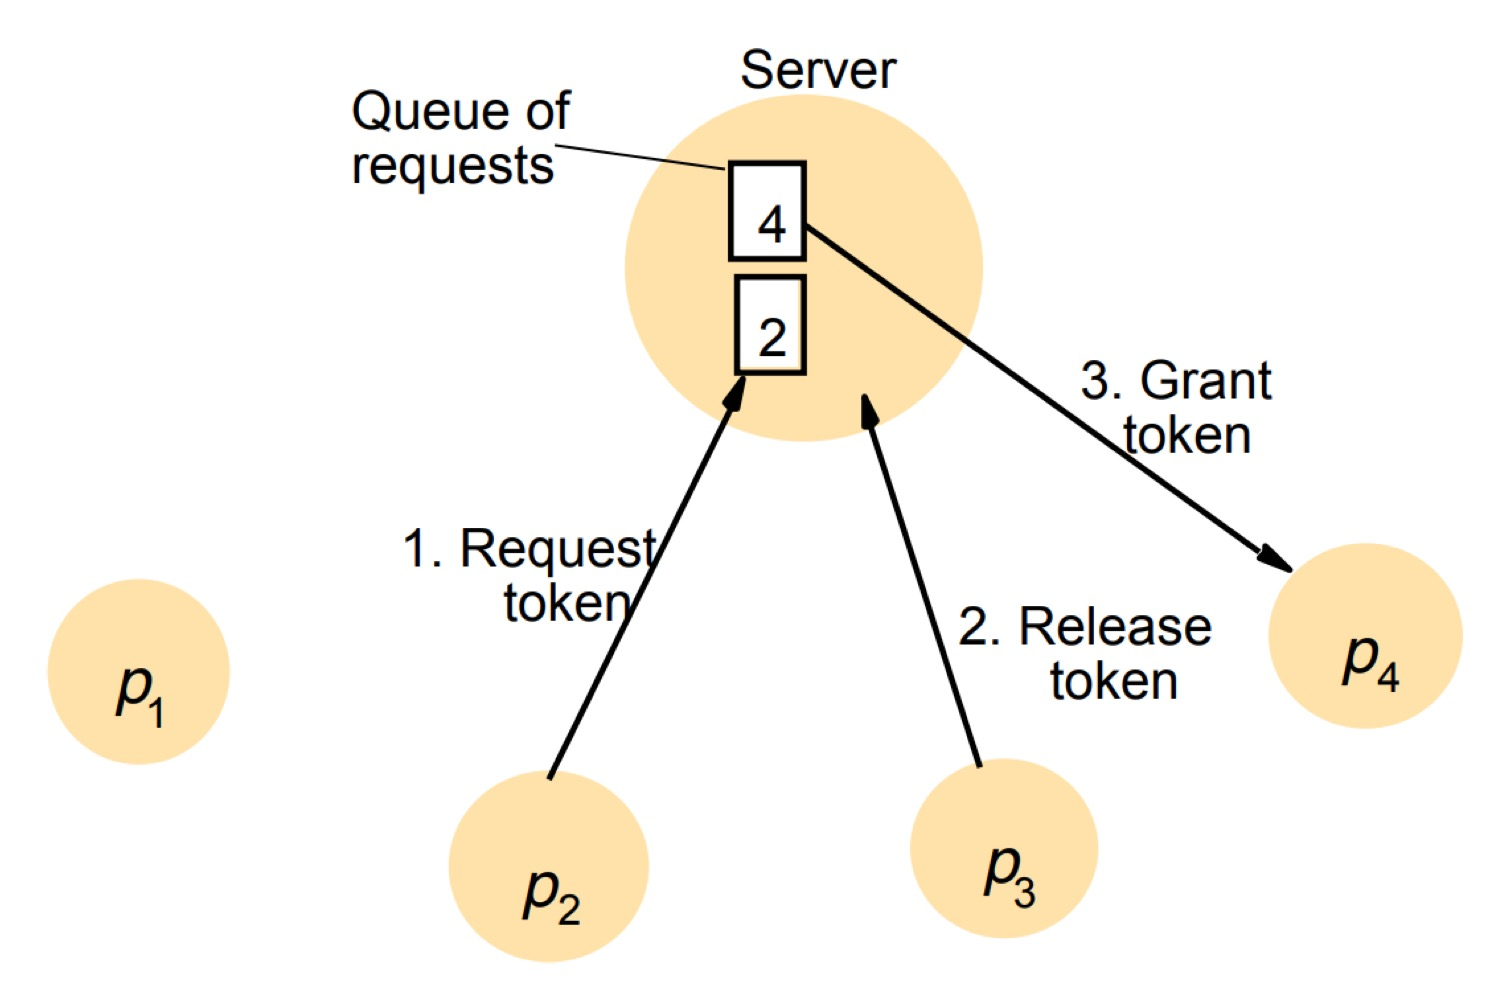
\includegraphics[width=.5\linewidth]{images/SynchronizationCoordinationDS/cebtralizedAlgorithm.jpeg}
    \caption{Server Managing a mutual exclusion token for a set of processes: Centralized Algorithm}
\end{figure}

\section{Distributed Algorithm}
DA works under the assumption that there exists a \textbf{global ordering of events}, normally each algorithm is based like so:
\begin{itemize}
    \item Protocol to \textbf{enter / exit to the critical section:}
        \begin{itemize}
            \item A process that wants to \textbf{enter a critical section} sends a message to all the other process, via \textit{multicast} with the \textbf{name} of the critical section, \textbf{its own identifier} and the \textbf{local timestamp}
            \item It \textbf{waits} for the answer from all the processes
            \item Once all the \textbf{OK have been received}, it \textbf{enters} the critical section
            \item At the \textbf{exit time} from the critical section, it sends \textbf{OK to all the processes in the local queue}
        \end{itemize}
    \item Protocol to \textbf{receive a request}
        \begin{itemize}
            \item Be \textbf{out of the critical section and it does not want to enter} \(\rightarrow\) sends \textbf{OK to the sender}
            \item \textbf{Be in the critical section} \(\rightarrow\) it does not answer and put \textbf{message in a local queue}
            \item \textbf{Wants to enter in the critical section} \(\rightarrow\) compares the \textbf{timestamp} and the \textbf{oldest has higher priority}, if it is the oldest process, it sends the \textbf{OK}, otherwise, if it is itself, it put \textbf{the message in the local queue}
        \end{itemize}
\end{itemize}

\begin{figure}[!h]
    \centering
    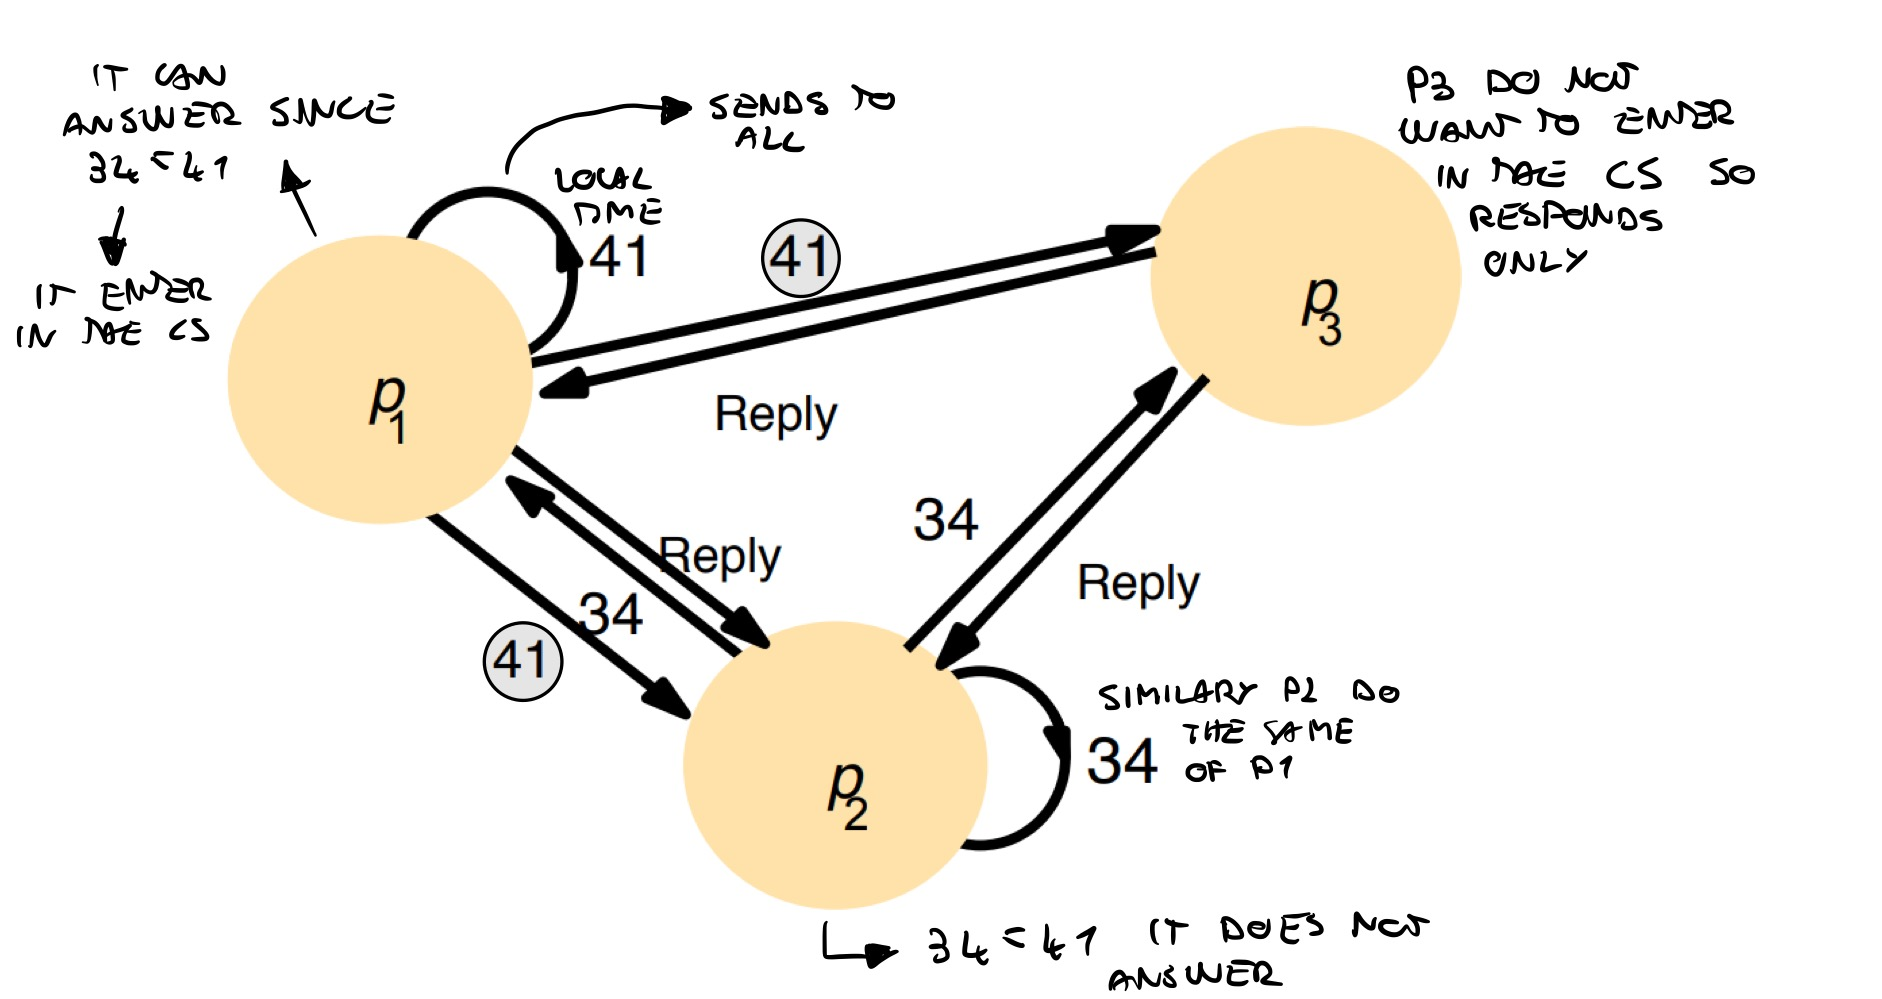
\includegraphics[width=.7\linewidth]{images/SynchronizationCoordinationDS/multicastSynch.jpeg}
    \caption{Multicast Synchronization}
\end{figure}

This algorithm satisfies all the three mutual exclusion criteria, but it has some \textbf{drawbacks:}
\begin{itemize}
    \item \textbf{High traffic} generated by \(N\) processes that require \(2(N - 1)\) messages for the multicast request and the answer
    \item \textbf{Fault of the system} if one of the processes crashed
    \item \textbf{Possible bottleneck} introduced by processes
\end{itemize}

\section{Ring Algorithm}
Processes share a \textbf{token} using a \textbf{local ring} structure. 
\begin{enumerate}
    \item The first process has a \textbf{token} that uses and then forwards to the next one.
    \item The process that \textbf{has the token} is enable to \textbf{access to the critical section}.
\end{enumerate} 
This algorithm satisfies the \textit{Safety} and \textit{liveness} conditions but not the \textit{ordering} one. It has the following features:
\begin{itemize}
    \item \textbf{Costs:} \([1, N - 1]\) messages to obtain the token. 1 message to exit fro the critical section and \([1, N - 1]\) message for synchronization
    \item \textbf{Reliability:} 
    \begin{itemize}
        \item If a process faults it is necessary to \textbf{rebuild the logical ring}
        \item If a process having the token faults it is necessary to make an \textbf{election} of the next process that will have the token
        \item Loss of the token also for hardware/software faults
    \end{itemize}
    \item \textbf{Performance:} the algorithm always \textbf{requires bandwidth to transmit the token} even if none ask for the critical section
\end{itemize}

\begin{figure}[!h]
    \centering
    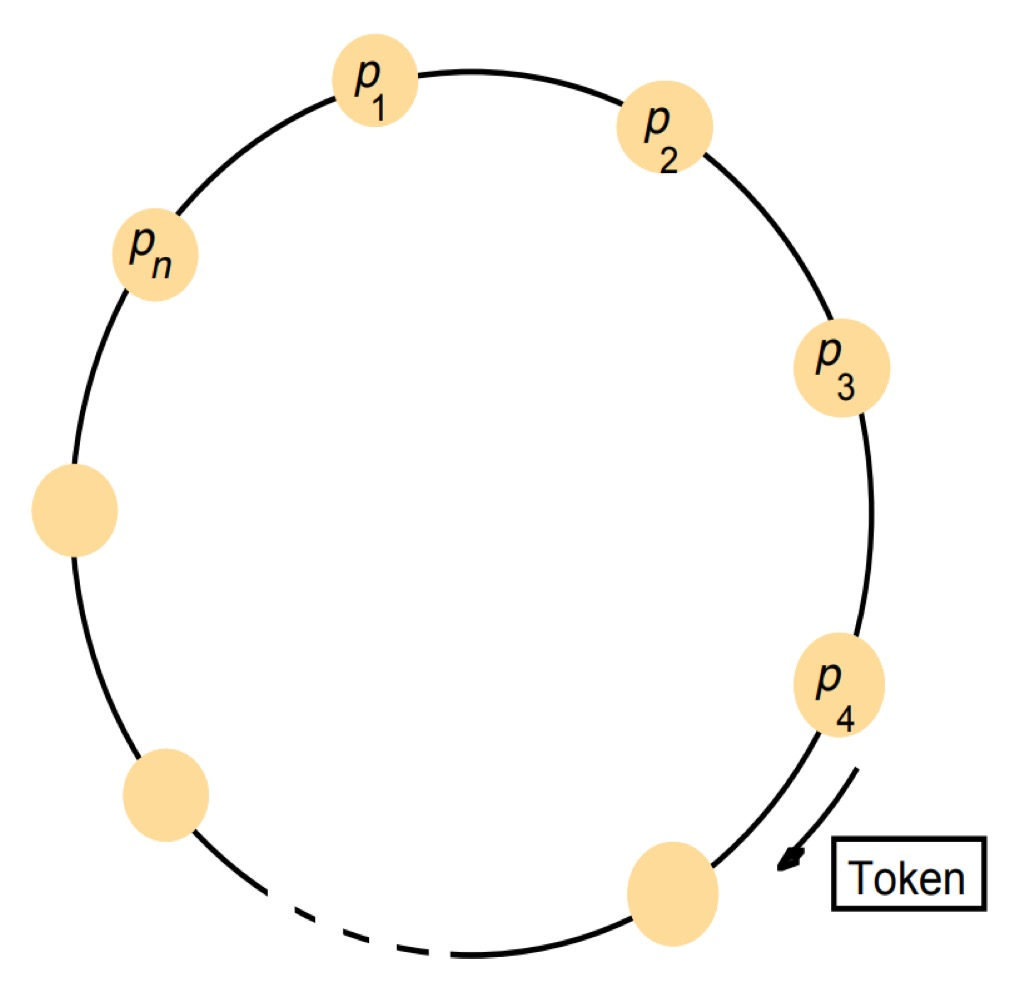
\includegraphics[width=.5\linewidth]{images/SynchronizationCoordinationDS/ringMutialExclusionToken.jpeg}
    \caption{A ring of process transferring a mutual exclusion token}
\end{figure}

\newpage
\section{Voting Algorithm}
In order to enter in the critical section, it is necessary to \textbf{synchronize only a subset of the interested processes.} So the processes make a vote (\textit{election}) to decide which process can access to the critical section:
\begin{itemize}
    \item Vote set \(V_i\) is a subset of \({p_1,...,p_N}\), associated to each process \(p_i\)
    \item A process that wants to \textbf{enter in the critical section} sends a message to all the other processes in \(V_i\)
    \item It \textbf{waits} for all the \textbf{replay}
    \item Once all the \textbf{OK} have been received it enters the critical section
    \item At the \textbf{exit time} from the critical section, it sends a message \textbf{release} to all the others members of \(V_i\)
    \item A process \(p_j\) in \(V_i\) that receives the request \(\rightarrow\) if its states is \textbf{HELD} or it \textbf{already answered} after having received the last message \textbf{release}, it does not answer and put the request in a \textbf{local queue}, otherwise it immediately answer with a \textbf{reply}
    \item A process that receives a \textbf{release} takes a requests from the queue and sends a \textbf{replay}
\end{itemize}

\newpage
\section{Comparison}
\begin{figure}[!h]
    \centering
    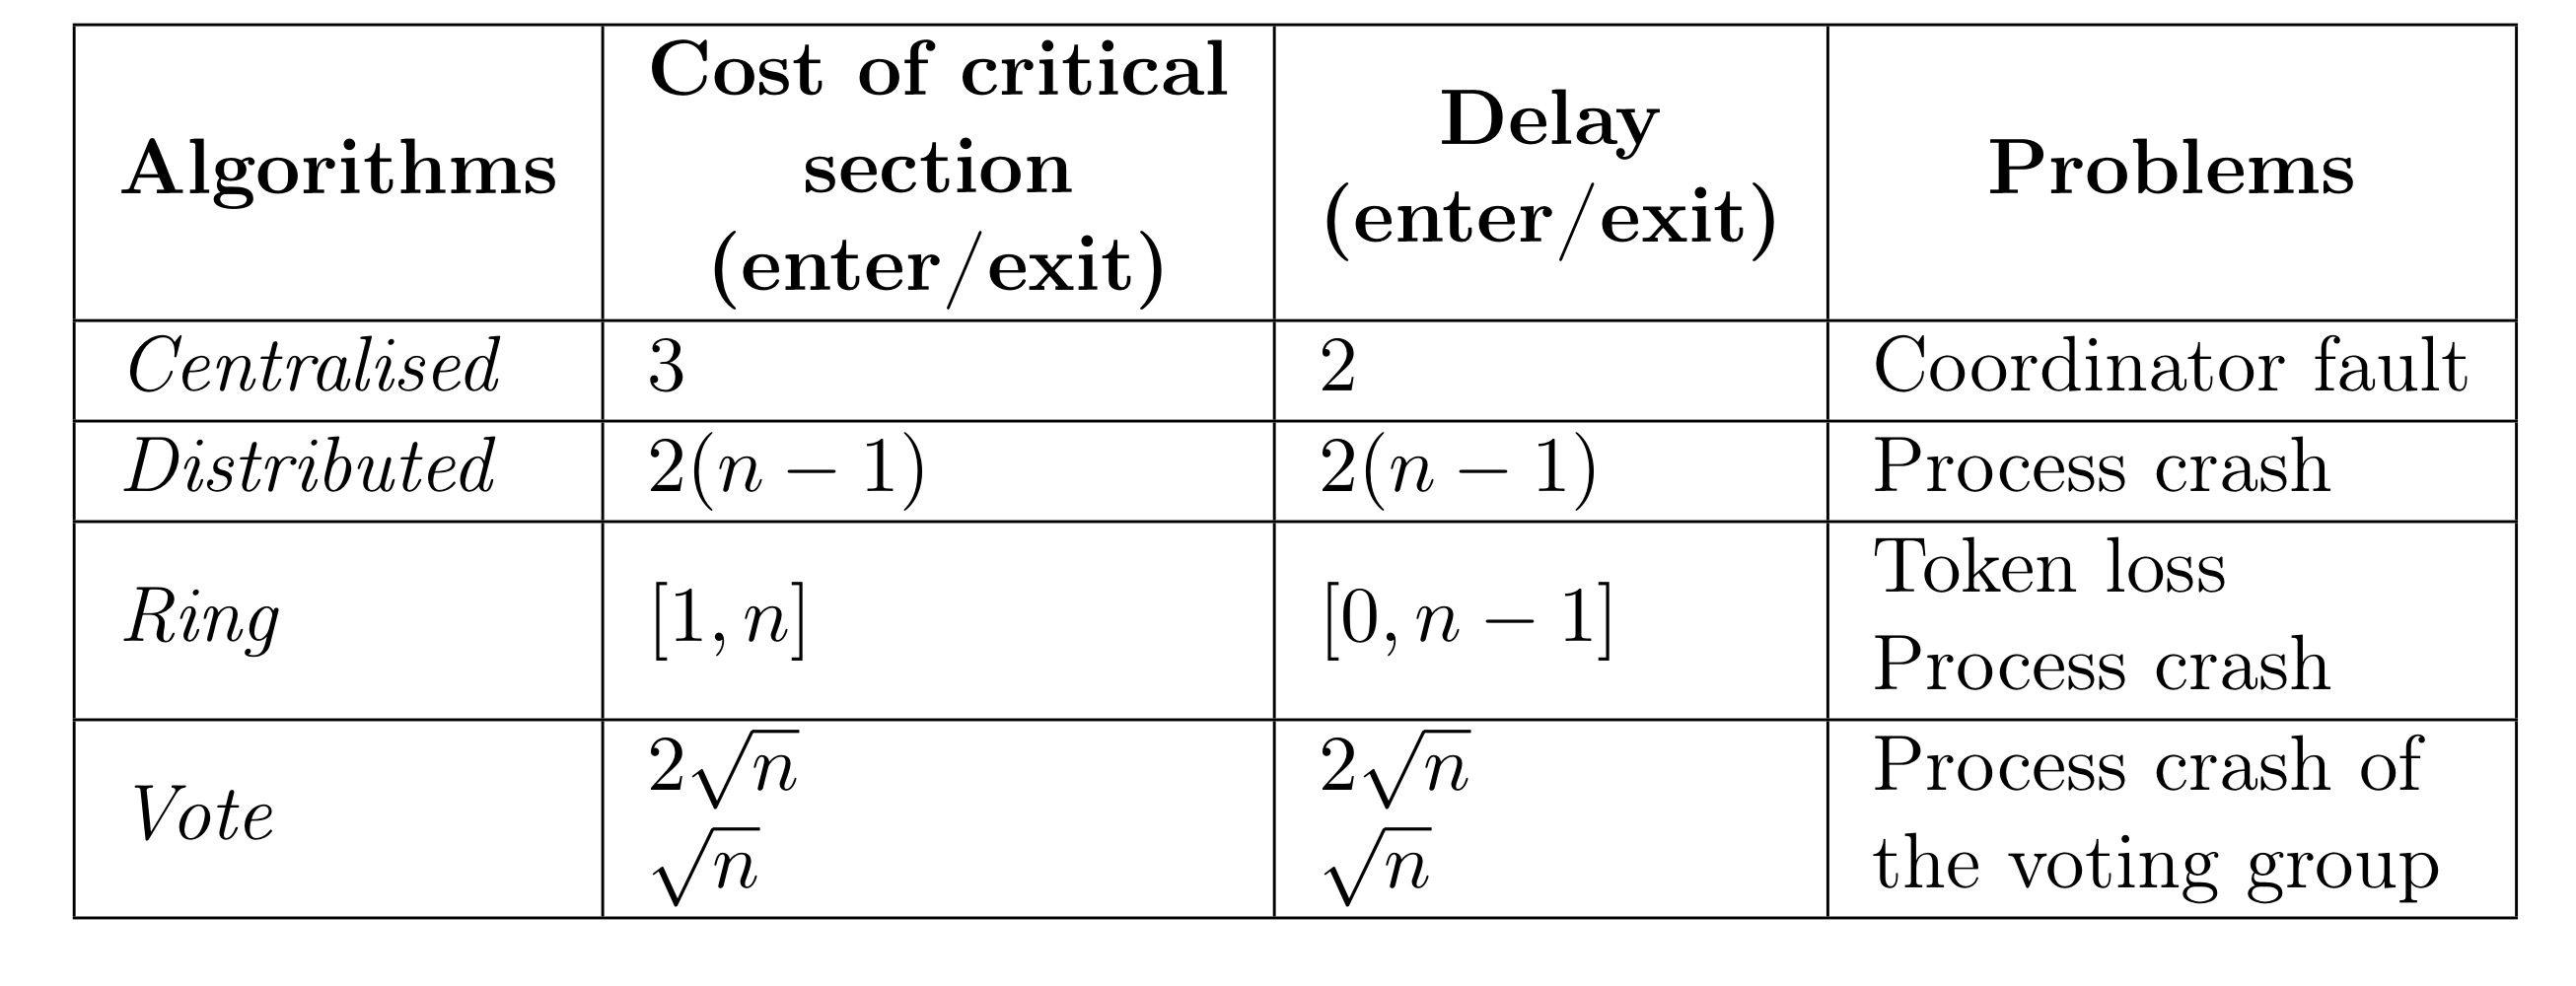
\includegraphics[width=.8\linewidth]{images/SynchronizationCoordinationDS/table.jpeg}
\end{figure}

\section{Election Algorithm}
The main goal of this algorithm is to let know all the processes on a specific \textbf{elected process} that act as \textbf{coordinator} in the distributed system. The following algorithm make three assumptions:
\begin{itemize}
    \item All the process are \textbf{uniquely numbered}
    \item The \textbf{coordinator} has usually the \textbf{highest number} among the process
    \item Each process knows the \textbf{number} of all the other processes 
\end{itemize}
Normally, a process calls an election and at the end of the algorithm, all the process agrees \textbf{on the same elected process}
The general structure of these algorithms is the following:
\begin{itemize}
    \item A process calls an election;
    \item Each process can be participant or not to the election;
    \item The elected process is unique even if more than one process called election.
\end{itemize}

\subsection{Circular Ordering}
It is structured as a logical ring composed by an ordered list of live processes in which the election message is sent only to the next process. It works as follow:
\begin{itemize}
    \item Every process at the beginning is \textbf{non participant}, it will become \textbf{participant} adding its name to the list
    \item If the election message ID is \textbf{greater}, it passes and becomes participant
    \item If the election message ID is \textbf{smaller}, it put its own id and passes
    \item If the election message ID is \textbf{the same}, then is a \textbf{coordinator}, it becomes \textbf{non participant}, and it sends an \textbf{elected} message
    \item Every other processes that receives an \textbf{elected} message are marked as non participant
\end{itemize}

\begin{figure}[!h]
    \centering
    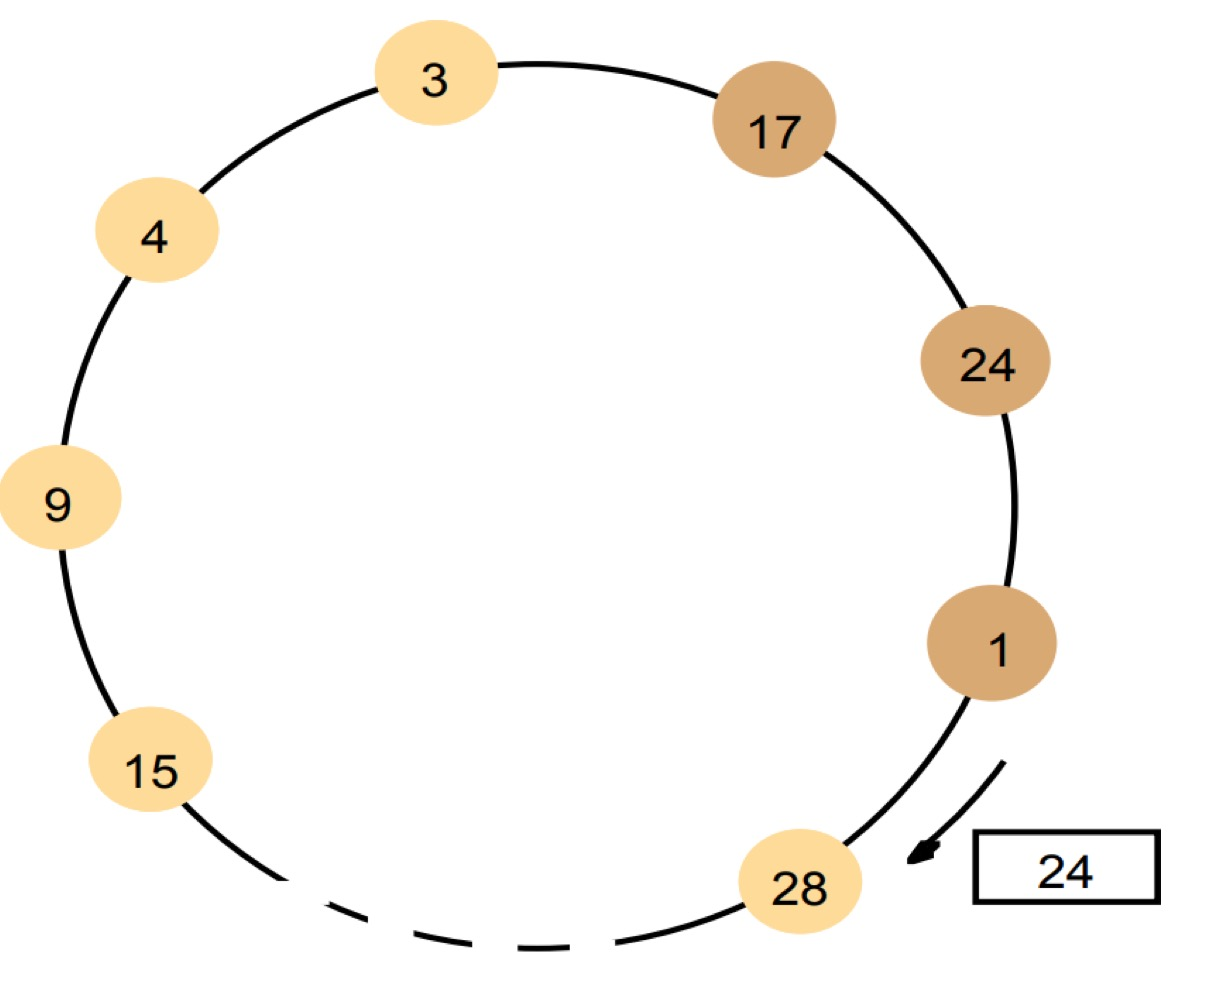
\includegraphics[width=.5\linewidth]{images/SynchronizationCoordinationDS/ringBasedElection.jpeg}
    \caption{A Ring-Based Election in process}
\end{figure}

\section{The Bully Algorithm}
In this algorithm each process communicate with process having \textbf{higher ID}. The message that are shared a are: \textit{election, answer} and \textit{coordinator}. It works as follow:
\begin{itemize}
    \item A process starts the election by sending an \textbf{election message} to all the process with \textbf{higher ID}, and waits for the replies
    \item If the \textbf{reply} does not arrive \textbf{within a timeout} a coordinator is nominated and communicate the news to the other processes
    \item Otherwise it \textbf{waits} for the arrival of a coordinator message and if it \textbf{does not arrive}, starts another election
    \item A process that \textbf{receives a coordinator message} saves the number and consider that process as \textbf{coordinator}
    \item A process that \textbf{receives} an election message sends a \textbf{reply} to the \textbf{sender} and starts a \textbf{new election}, unless it has already done it. 
\end{itemize}
\begin{figure}[!h]
    \centering
    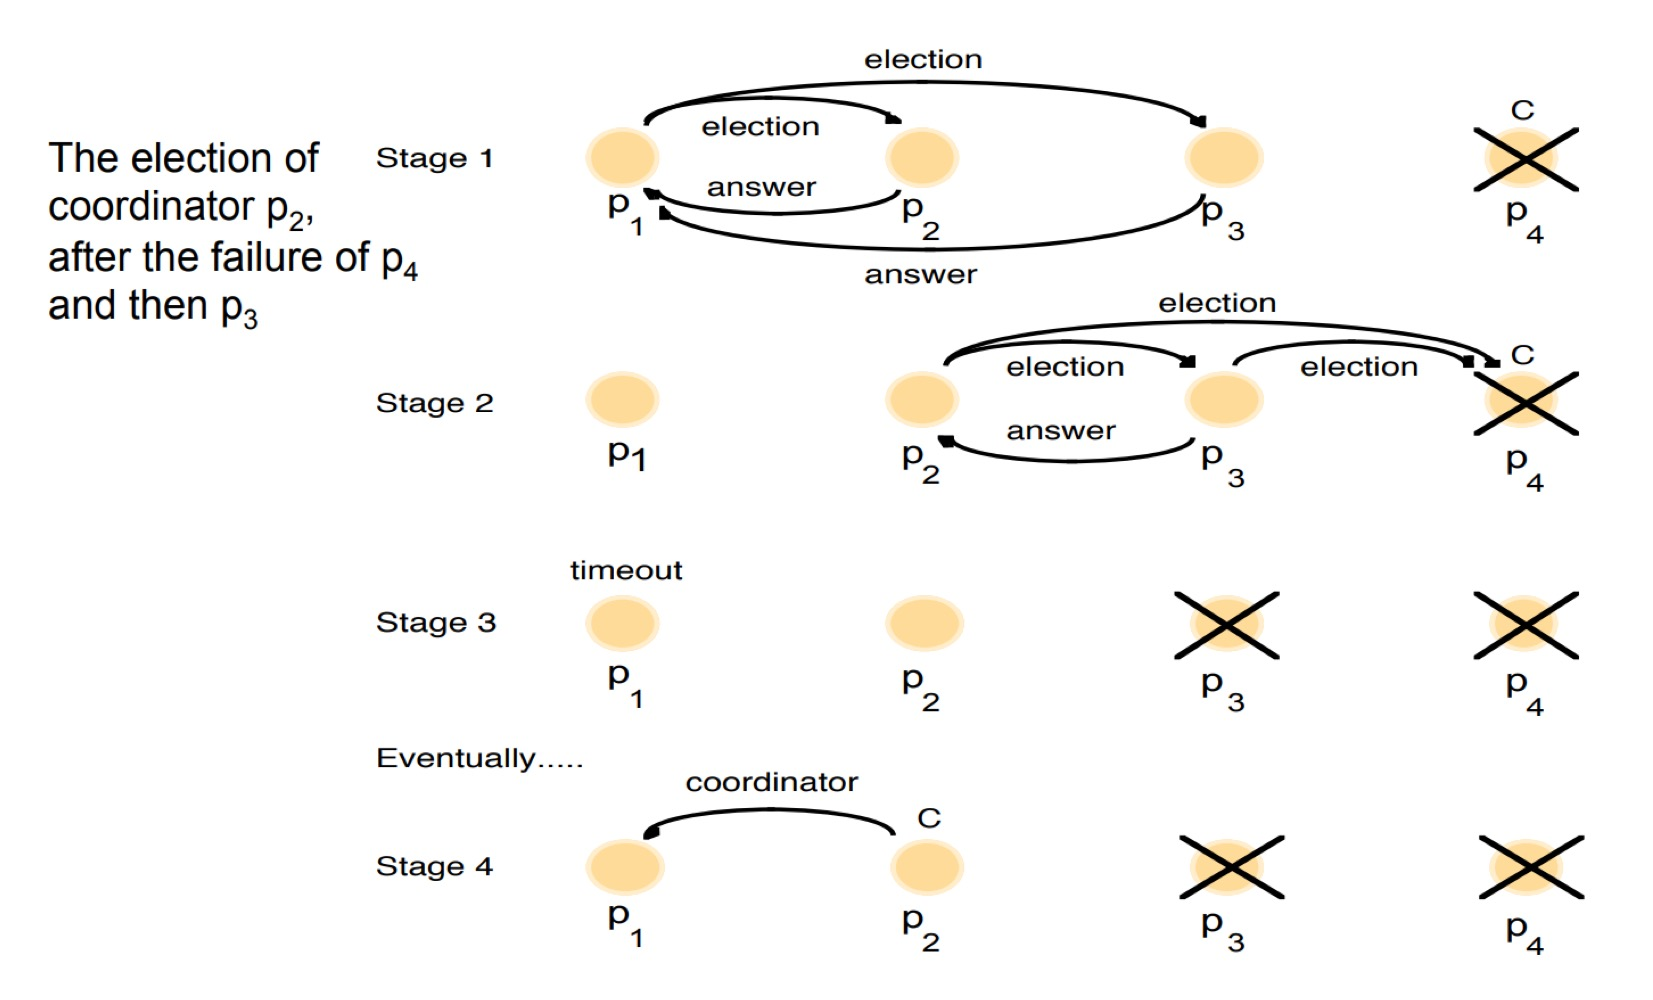
\includegraphics[width=.9\linewidth]{images/SynchronizationCoordinationDS/bullyAlgorithm.jpeg}
    \caption{Example of execution of Bully Algorithm}
\end{figure}
A process \textbf{starts an election} in the following cases:
\begin{itemize}
    \item When a process is reactivated after a faults
    \item When a process realizes that the coordinator does not answer
    \item When a process receives an election message from a process with lower ID
\end{itemize}
The Bully Algorithm has the following cost performance:
\begin{itemize}
    \item \textbf{Worst case:} \(O(n^2)\) messages
    \item \textbf{Best case:} \(O(n - 1)\) messages
\end{itemize}


\section{Deadlock Management}
Deadlock could be a side effect of the \textbf{mutual exclusion}. It could happen because of:
\begin{itemize}
    \item \textbf{Resource allocation without pre-emption:} the system cannot force a process to release a resource
    \item \textbf{Hold and wait:} a process that holds a resource keeps holding it
    \item \textbf{Circular waiting:} there exists a closed path in the allocation graph
\end{itemize}
\begin{figure}[!h]
    \centering
    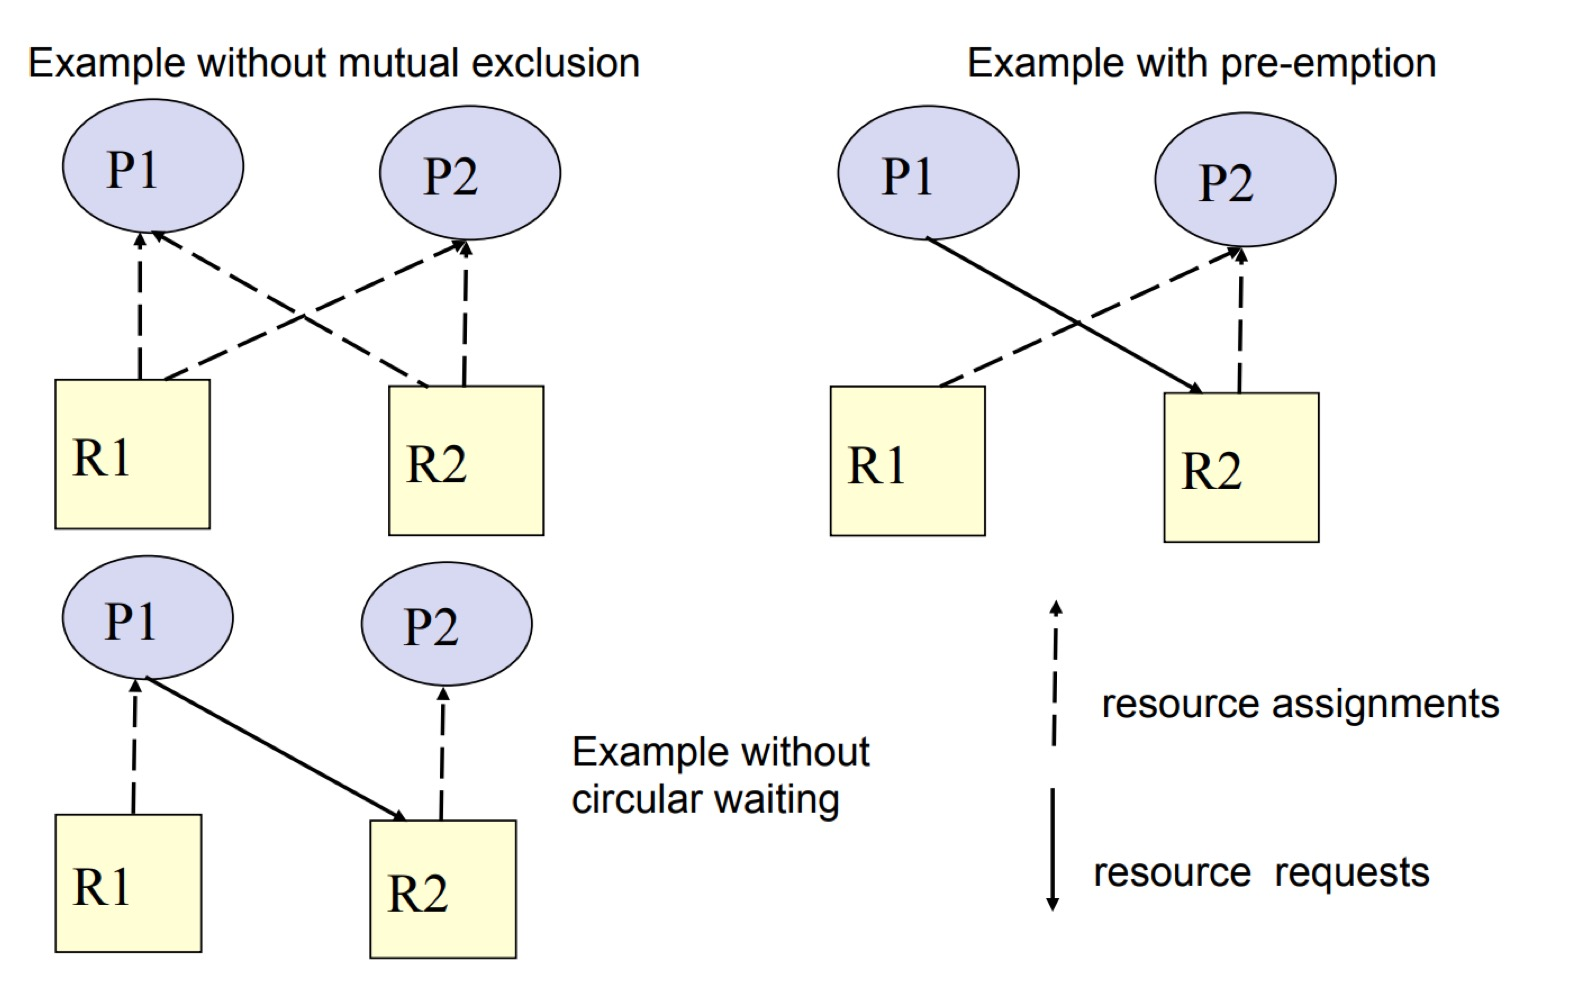
\includegraphics[width=.8\linewidth]{images/SynchronizationCoordinationDS/deadlock.jpeg}
    \caption{Deadlock Conditions}
\end{figure}
There are \textbf{different types} of deadlock:
\begin{itemize}
    \item \textbf{Communication deadlock:} if the resource is a buffer
    \item \textbf{Direct store and Forward store:} if it involves two nodes
    \item \textbf{Indirect store and Forward store:} if it involves \textit{more than} two nodes
\end{itemize}

In order to manage the possible presence of deadlock a \textbf{PAID} technique is used \textit{(Prevent - Avoid - Ignore - Detect)}:
\begin{itemize}
    \item \textbf{Prevention} applied by:
        \begin{itemize}
            \item Allowing only one resource allocation
            \item Pre-allocate resources
            \item Ordering
            \item Age rule
        \end{itemize}
    \item \textbf{Avoidance:} it determines the stable states on the basis of the process needs
    \item \textbf{Ignoring:} applied to terminate process in cyclic waiting
    \item \textbf{Detection:} by applying \textit{Chandy-Misra-Haas} algorithm:
        \begin{enumerate}
            \item A blocked process \(P_1\) starts a test (structure composed of \[ID_{blocked process}, ID_{sending test process}, ID_{receiving test process}\]
            \item \(P_2\) receives the test and if it does not need other resources it stops the test. Otherwise if it is blocked by \(P_3\) it forward the test
            \item If a process receives a test with \(ID_{blocked process} = ID_{receiving test process}\) it detects the deadlock
        \end{enumerate}
\end{itemize}